% Options for packages loaded elsewhere
\PassOptionsToPackage{unicode}{hyperref}
\PassOptionsToPackage{hyphens}{url}
%
\documentclass[
]{article}
\usepackage{amsmath,amssymb}
\usepackage{iftex}
\ifPDFTeX
  \usepackage[T1]{fontenc}
  \usepackage[utf8]{inputenc}
  \usepackage{textcomp} % provide euro and other symbols
\else % if luatex or xetex
  \usepackage{unicode-math} % this also loads fontspec
  \defaultfontfeatures{Scale=MatchLowercase}
  \defaultfontfeatures[\rmfamily]{Ligatures=TeX,Scale=1}
\fi
\usepackage{lmodern}
\ifPDFTeX\else
  % xetex/luatex font selection
\fi
% Use upquote if available, for straight quotes in verbatim environments
\IfFileExists{upquote.sty}{\usepackage{upquote}}{}
\IfFileExists{microtype.sty}{% use microtype if available
  \usepackage[]{microtype}
  \UseMicrotypeSet[protrusion]{basicmath} % disable protrusion for tt fonts
}{}
\makeatletter
\@ifundefined{KOMAClassName}{% if non-KOMA class
  \IfFileExists{parskip.sty}{%
    \usepackage{parskip}
  }{% else
    \setlength{\parindent}{0pt}
    \setlength{\parskip}{6pt plus 2pt minus 1pt}}
}{% if KOMA class
  \KOMAoptions{parskip=half}}
\makeatother
\usepackage{xcolor}
\usepackage[margin=1in]{geometry}
\usepackage{graphicx}
\makeatletter
\def\maxwidth{\ifdim\Gin@nat@width>\linewidth\linewidth\else\Gin@nat@width\fi}
\def\maxheight{\ifdim\Gin@nat@height>\textheight\textheight\else\Gin@nat@height\fi}
\makeatother
% Scale images if necessary, so that they will not overflow the page
% margins by default, and it is still possible to overwrite the defaults
% using explicit options in \includegraphics[width, height, ...]{}
\setkeys{Gin}{width=\maxwidth,height=\maxheight,keepaspectratio}
% Set default figure placement to htbp
\makeatletter
\def\fps@figure{htbp}
\makeatother
\setlength{\emergencystretch}{3em} % prevent overfull lines
\providecommand{\tightlist}{%
  \setlength{\itemsep}{0pt}\setlength{\parskip}{0pt}}
\setcounter{secnumdepth}{-\maxdimen} % remove section numbering
\ifLuaTeX
  \usepackage{selnolig}  % disable illegal ligatures
\fi
\IfFileExists{bookmark.sty}{\usepackage{bookmark}}{\usepackage{hyperref}}
\IfFileExists{xurl.sty}{\usepackage{xurl}}{} % add URL line breaks if available
\urlstyle{same}
\hypersetup{
  pdftitle={MLE},
  pdfauthor={Mu Lifeng},
  hidelinks,
  pdfcreator={LaTeX via pandoc}}

\title{MLE}
\author{Mu Lifeng}
\date{2020/4/18}

\begin{document}
\maketitle

\section{极大似然估计(MLE)}\label{ux6781ux5927ux4f3cux7136ux4f30ux8ba1mle}

在初中阶段的基础统计分析章节中,我们学习了一些描述数据集中趋势和波动情况(离散趋势)的统计指标,如平均数、中位数、方差和标准差等等。教材中给出了这样一些计算公式:
\[\bar{X} = \frac{\left(x_1+ x_2 + \cdots + x_n\right)}{n}\]
\[s^2 = \frac{[(x_1-\bar{x})^2+(x_2-\bar{x})^2+\cdots+(x_n-\bar{x})^2]}{n}\]
\[s = \sqrt{\frac{1}{n}[(x_1-\bar{x})^2 + (x_2-\bar{x})^2 + \cdots + (x_n-\bar{x})^2]}\]

若一组数据服从正态分布,上述公式则正好为正态分布参数的极大似然估计。这些公式看起来是理所当然的,实际上我们可以通过数学方法来证明它。

极大似然估计是在给定数据的情况下,推断最有可能的参数分布。也就是说,极大似然估计的工作就是找到一个概率分布(包括概率分布形式、分布参数),使其能够最好地描述所获得的数据。以正态分布为例,正态分布的概率密度函数为:
\[f(x)=\frac{1}{\sqrt{2\pi}\sigma}\exp(-\frac{(x-\mu)^2}{2\sigma^2})\]

标准正态分布概率密度函数图

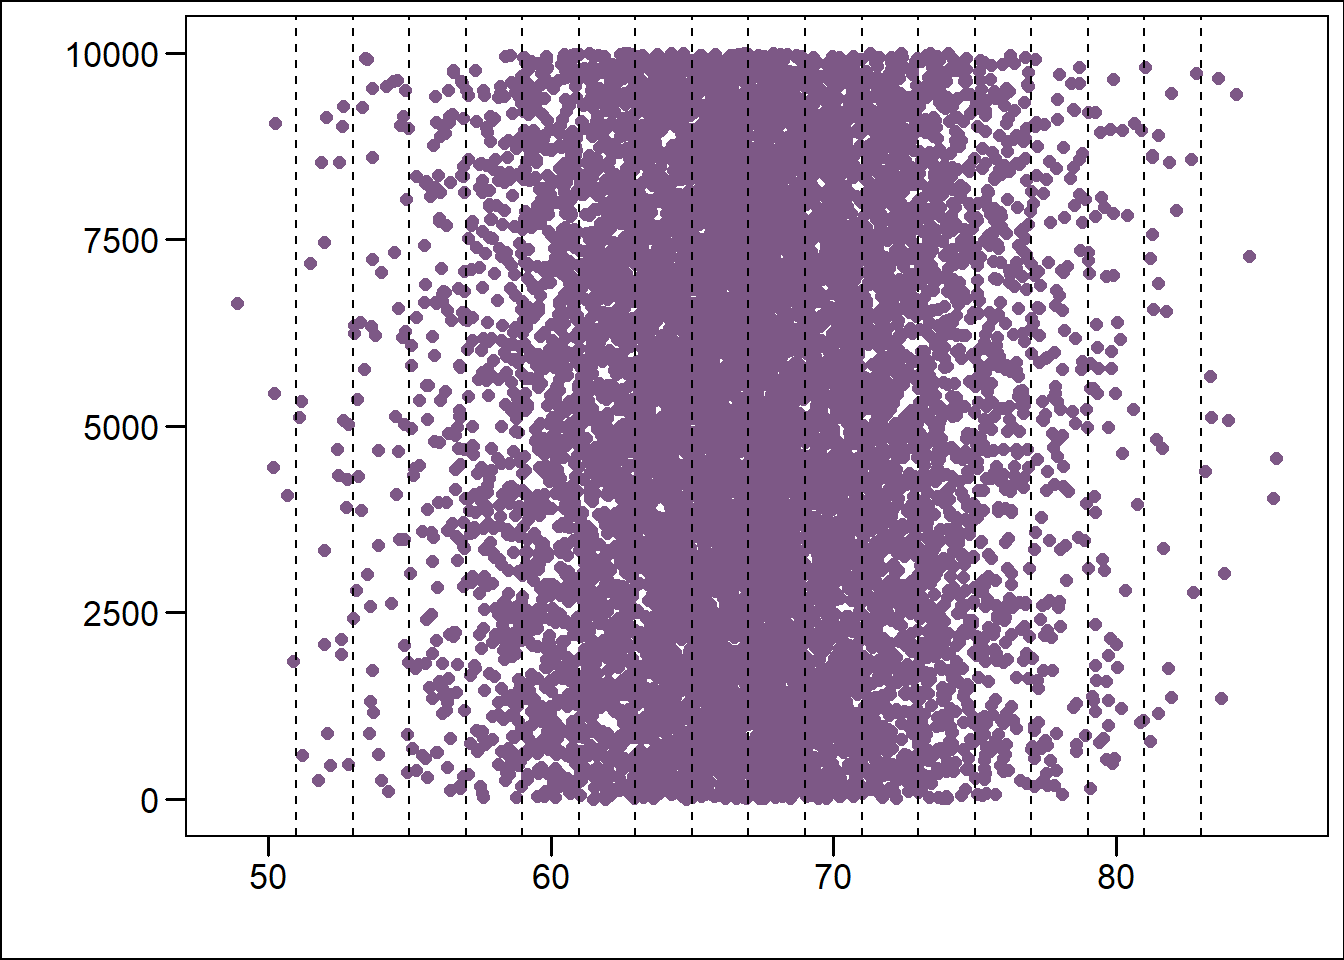
\includegraphics{MLE_files/figure-latex/unnamed-chunk-1-1.pdf}

如果我们获得了一份包含n个值的样本,数据服从均值为μ,方差为\(σ^2\)的正态分布:
\[x_1, x_2, x_3, \cdots, x_n\]

根据正态概率密度函数可以写出其似然函数为:
\[L(\mu,\sigma \mid x)=\frac{1}{\sqrt{2\pi}\sigma}\exp(-\frac{(x-\mu)^2}{2\sigma^2})\]
接下来就是求出使得\(L(\mu,\sigma \mid X)\)取最大值的\(\mu\)和\(\sigma\)。可通过求二阶偏导数求得该二元函数的最值。
在求导之前先两边同时取对数,以利于求导计算。即: \[
\begin{align}
\ln L(\mu,\sigma \mid x)&=\ln (\frac{1}{\sqrt{2\pi}\sigma}\exp(-\frac{(x-\mu)^2}{2\sigma^2})) \\
&= \ln(\frac{1}{\sqrt{2\pi}\sigma}) -\frac{(x-\mu)^2}{2\sigma^2} \\
&=  0-\ln (\sqrt{2\pi}\sigma)-\frac{(x-\mu)^2}{2\sigma^2}\\
&= -\ln(\sqrt{2\pi}) - \ln (\sigma) - \frac{(x-\mu)^2}{2\sigma^2} \\
\end{align}
\] 此时,可求\(\mu\)的偏导数: \[
\begin{align}
\frac{\partial{\ln L(\mu,\sigma \mid x)}}{\partial{\mu}} &= -0-0-\frac{2(x-\mu)}{2\sigma^2}(-1)\\
&= \frac{x-\mu}{\sigma^2}
\end{align}
\] 同样,可求得关于\(\sigma\)的偏导数: \[
\begin{align}
\frac{\partial{\ln L(\sigma,\mu \mid x)}}{\partial{\sigma}} &=
-0-\frac{1}{\sigma}-(-2)\frac{(x-\mu)^2}{2}\sigma^{-3} \\ 
&= -\frac{1}{\sigma}+\frac{(x-\mu)^2}{\sigma^3} \\
\end{align}
\]

根据:
\[L(\mu,\sigma \mid X)=L(\mu,\sigma \mid x_1)L(\mu,\sigma \mid x_2)L(\mu,\sigma \mid x_3) \cdots L(\mu,\sigma \mid x_n)\]
可得: \[
\begin{align}
\ln L(\mu,\sigma \mid X)&=\ln L(\mu,\sigma \mid x_1)+\ln L(\mu,\sigma \mid x_2)+\ln L(\mu,\sigma \mid x_3)+\cdots+\ln L(\mu,\sigma \mid x_n) \\
\end{align}
\] 所以: \[
\begin{align}
\frac{\partial{\ln L(\mu,\sigma \mid X)}}{\partial{\mu}} &= \frac{x_1-\mu}{\sigma^2} + \frac{x_2-\mu}{\sigma^2} + \frac{x_3-\mu}{\sigma^2} + \cdots + \frac{x_n-\mu}{\sigma^2} \\
&= \frac{(x_1-\mu) + (x_2-\mu) + (x_3-\mu) + \cdots + (x_n-\mu)}{\sigma^2} \\
&= \frac{(x_1+ x_2 + \cdots + x_n) - n\mu}{\sigma^2}
\end{align}
\] 令\(\frac{\partial{\ln L(\mu,\sigma \mid X)}}{\partial{\mu}}\) =
0,得: \[
\begin{align}
\frac{(x_1+ x_2 + \cdots + x_n) - n\mu}{\sigma^2} = 0 \\
(x_1+ x_2 + \cdots + x_n) = n\mu \\
\mu = \frac{(x_1+ x_2 + \cdots + x_n)}{n}
\end{align}
\]

\subsubsection{surprise!}\label{surprise}

\(\mu\)的极大似然估计值即为所有观察值的均数

同理:

\[
\begin{align}
\frac{\partial{\ln L(\mu,\sigma \mid x)}}{\partial{\sigma^2}}
&= -\frac{1}{\sigma}+\frac{(x_1-\mu)^2}{\sigma^3} -\frac{1}{\sigma}+\frac{(x_2-\mu)^2}{\sigma^3} -\frac{1}{\sigma}+\frac{(x_3-\mu)^2}{\sigma^3} - \cdots -\frac{1}{\sigma}+\frac{(x_n-\mu)^2}{\sigma^3} \\
&= -\frac{n}{\sigma} + \frac{(x_1-\mu)^2+(x_2-\mu)^2+(x_3-\mu)^2+\cdots+(x_n-\mu)^2}{\sigma^3}\\
\end{align}
\] 令\(\frac{\partial{\ln L(\mu,\sigma \mid x)}}{\partial{\sigma}}\) =
0,即得: \[
-\frac{n}{\sigma} + \frac{(x_1-\mu)^2+(x_2-\mu)^2+(x_3-\mu)^2+\cdots+(x_n-\mu)^2}{\sigma^3} = 0 \\
\frac{(x_1-\mu)^2+(x_2-\mu)^2+(x_3-\mu)^2+\cdots+(x_n-\mu)^2}{\sigma^2} = n \\
\sigma^2 = \frac{(x_1-\mu)^2+(x_2-\mu)^2+(x_3-\mu)^2+\cdots+(x_n-\mu)^2}{n}
\]

\subsubsection{surprise!}\label{surprise-1}

显然,上述数据也可能不服从正态分布,那么同样的思路可以用于求解其它概率分布参数的极大似然估计值:写出似然函数、求导(先取对数)、令导数值为0求解。

如果数据服从指数分布\(f(x)=\lambda e^{(-\lambda x)}\),利用上述方法可求得参数\(\lambda\)的极大似然估计值为:
\[\lambda=\frac{x}{x_1+x_2+\cdots+x_n}\]
又如,当数据服从二项分布\(f(x)=\binom{x}{n}p^k(1-p)^{n-x}\)时,其参数\(p\)的极大似然估计为:
\[p=\frac{x}{n}\]

\subsection{References}\label{references}

本文是对\href{https://www.youtube.com/watch?v=XepXtl9YKwc}{StatQuest}中有关内容的整理和复现

\end{document}
